\documentclass[tikz,border=0pt]{standalone}
\usepackage{fontspec}
\usepackage{amsmath}
\usepackage{xcolor}
\usepackage{tikz}
\usepackage{pgfplots}
\pgfplotsset{compat=1.18}
\usetikzlibrary{arrows.meta,calc,fit,positioning,shapes.geometric,shapes.misc,patterns,plotmarks}
\IfFontExistsTF{Arial}{\setsansfont{Arial}}{\setsansfont{TeX Gyre Heros}}
\renewcommand{\familydefault}{\sfdefault}
\tikzset{
  >={Stealth[length=2.2mm,width=1.5mm]},
  exact title/.style={font=\bfseries\fontsize{10.5}{12}\selectfont,align=center},
  exact subtitle/.style={font=\fontsize{6.3}{7.2}\selectfont,align=center},
  exact label/.style={font=\fontsize{6.4}{7.5}\selectfont,align=center},
  exact tiny/.style={font=\fontsize{5.3}{6.3}\selectfont,align=center},
  panel/.style={draw=black!14,rounded corners=1.2mm,fill=white,line width=.45pt},
  neutral/.style={draw=black!30,fill=black!3,rounded corners=1mm,line width=.45pt},
  arrow/.style={-Stealth,line width=.7pt},
  softarrow/.style={-Stealth,line width=.55pt,draw=black!45},
  dashedarrow/.style={-Stealth,dashed,line width=.55pt,draw=black!55},
  metric/.style={font=\fontsize{5.3}{6.3}\selectfont,fill=white,inner sep=1pt},
}
\newcommand{\pill}[4]{\node[draw=#2!70,fill=#2!10,rounded corners=1.5mm,inner xsep=3pt,inner ysep=2pt,exact label,text=#2] (#1) at #3 {#4};}
\newcommand{\frameboxx}[4]{\draw[draw=#2!65,fill=#2!8,rounded corners=.6mm,line width=.5pt] (#1.south west) rectangle (#1.north east);\node[exact tiny,text=#2] at #3 {#4};}
\newcommand{\axislabel}[3]{\node[exact tiny,text=black!60] at (#1) {#2};\node[exact tiny,text=black!60,rotate=90] at (#3) {#2};}

\definecolor{mgreen}{HTML}{96E696}\definecolor{morange}{HTML}{FF7F0E}\definecolor{mpurple}{HTML}{C58EF7}\definecolor{mlightblue}{HTML}{79C4F7}\definecolor{mcharcoal}{HTML}{3A3A3A}
\begin{document}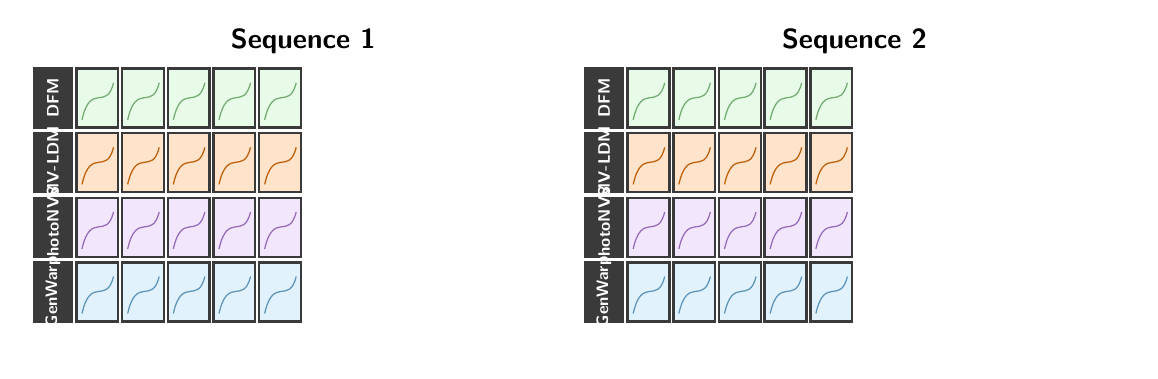
\begin{tikzpicture}[x=1cm,y=1cm]
\path[use as bounding box] (0,0) rectangle (14,4.1);
\node[font=\bfseries\fontsize{10}{11}\selectfont] at (3.5,3.92) {Sequence 1};\node[font=\bfseries\fontsize{10}{11}\selectfont] at (10.5,3.92) {Sequence 2};
\foreach \r/\lab/\c in {0/DFM/mgreen,1/MV-LDM/morange,2/PhotoNVS/mpurple,3/GenWarp/mlightblue}{\draw[draw=mcharcoal,fill=mcharcoal,line width=.9pt] (.08,3.58-\r*.82) rectangle (.56,2.83-\r*.82);\node[rotate=90,font=\bfseries\fontsize{6}{6}\selectfont,text=white] at (.32,3.205-\r*.82) {\lab};\foreach \j in {0,1,2,3,4}{\draw[draw=mcharcoal,fill=\c!22,line width=.9pt] (.62+\j*.58,2.83-\r*.82) rectangle (1.15+\j*.58,3.58-\r*.82);\draw[\c!75!black,line width=.45pt] (.69+\j*.58,2.93-\r*.82) .. controls (.8+\j*.58,3.42-\r*.82) and (1.0+\j*.58,3.03-\r*.82) .. (1.09+\j*.58,3.4-\r*.82);}\draw[draw=mcharcoal,fill=mcharcoal,line width=.9pt] (7.08,3.58-\r*.82) rectangle (7.56,2.83-\r*.82);\node[rotate=90,font=\bfseries\fontsize{6}{6}\selectfont,text=white] at (7.32,3.205-\r*.82) {\lab};\foreach \j in {0,1,2,3,4}{\draw[draw=mcharcoal,fill=\c!22,line width=.9pt] (7.62+\j*.58,2.83-\r*.82) rectangle (8.15+\j*.58,3.58-\r*.82);\draw[\c!75!black,line width=.45pt] (7.69+\j*.58,2.93-\r*.82) .. controls (7.8+\j*.58,3.42-\r*.82) and (8.0+\j*.58,3.03-\r*.82) .. (8.09+\j*.58,3.4-\r*.82);}}
\end{tikzpicture}\end{document}
